\begin{figure}[t]
\centering
\begin{tikzpicture}
\begin{axis}[width=0.5\textwidth,height=5.4cm,xmode=log,ymode=log,log basis x=2,xlabel={depth $L$},ylabel={normalized error $q_L$},
legend style={font=\scriptsize,at={(0.03,0.97)},anchor=north west,draw=none,fill=none},xtick={1,2,4,8,16,32,64},xticklabels={1,2,4,8,16,32,64},tick label style={font=\scriptsize},label style={font=\small}]
\addplot[black,thick] coordinates {(1,0.01) (2,0.0201) (3,0.030301) (4,0.040604) (6,0.0615202) (8,0.0828567) (12,0.126825) (16,0.172579) (24,0.269735) (32,0.374941) (48,0.612226) (64,0.890462)};
\addlegendentry{no compensation}
\addplot[black,only marks,mark=o,mark size=2.2pt,forget plot,error bars/.cd,y dir=both,y explicit] coordinates {(1,0.0100114) +- (0,3.13e-05) (2,0.0200965) +- (0,8.53e-05) (4,0.0405473) +- (0,0.000195) (8,0.0828237) +- (0,0.000445) (16,0.171966) +- (0,0.00107) (32,0.374935) +- (0,0.00288) (64,0.895835) +- (0,0.00963)};
\addplot[black,only marks,mark=x,mark size=2.6pt,forget plot,error bars/.cd,y dir=both,y explicit] coordinates {(1,0.00996622) +- (0,4.62e-05) (2,0.0201029) +- (0,0.000102) (4,0.0406934) +- (0,0.000212) (8,0.0829073) +- (0,0.00047) (16,0.172594) +- (0,0.00106) (32,0.374725) +- (0,0.00306) (64,0.883554) +- (0,0.01)};
\addplot[blue,thick] coordinates {(1,0.01) (2,0.0126) (3,0.013276) (4,0.0134518) (6,0.0135093) (8,0.0135132) (12,0.0135135) (16,0.0135135) (24,0.0135135) (32,0.0135135) (48,0.0135135) (64,0.0135135)};
\addlegendentry{$\alpha=\tfrac12$}
\addplot[blue,only marks,mark=o,mark size=2.2pt,forget plot,error bars/.cd,y dir=both,y explicit] coordinates {(1,0.0100216) +- (0,3.17e-05) (2,0.0126212) +- (0,4.95e-05) (4,0.0134319) +- (0,5.67e-05) (8,0.0135095) +- (0,5.63e-05) (16,0.013545) +- (0,5.67e-05) (32,0.0135087) +- (0,5.68e-05) (64,0.0135269) +- (0,5.58e-05)};
\addplot[blue,only marks,mark=x,mark size=2.6pt,forget plot,error bars/.cd,y dir=both,y explicit] coordinates {(1,0.00994729) +- (0,4.76e-05) (2,0.0125954) +- (0,6.1e-05) (4,0.0134065) +- (0,6.98e-05) (8,0.0135752) +- (0,7.74e-05) (16,0.0134728) +- (0,7.76e-05) (32,0.0135408) +- (0,8.22e-05) (64,0.0135738) +- (0,8.47e-05)};
\addplot[red,thick] coordinates {(1,0.01) (2,0.0101) (3,0.010101) (4,0.010101) (6,0.010101) (8,0.010101) (12,0.010101) (16,0.010101) (24,0.010101) (32,0.010101) (48,0.010101) (64,0.010101)};
\addlegendentry{$\alpha=1$}
\addplot[red,only marks,mark=o,mark size=2.2pt,forget plot,error bars/.cd,y dir=both,y explicit] coordinates {(1,0.00999414) +- (0,3.17e-05) (2,0.0101162) +- (0,3.34e-05) (4,0.0100873) +- (0,3.35e-05) (8,0.0101175) +- (0,3.35e-05) (16,0.0101065) +- (0,3.35e-05) (32,0.0101146) +- (0,3.36e-05) (64,0.010097) +- (0,3.38e-05)};
\addplot[red,only marks,mark=x,mark size=2.6pt,forget plot,error bars/.cd,y dir=both,y explicit] coordinates {(1,0.00996923) +- (0,4.85e-05) (2,0.0101361) +- (0,4.64e-05) (4,0.0101182) +- (0,4.71e-05) (8,0.0101191) +- (0,4.52e-05) (16,0.010034) +- (0,5.07e-05) (32,0.0100701) +- (0,5.56e-05) (64,0.0101319) +- (0,4.82e-05)};
\end{axis}
\end{tikzpicture}\hfill
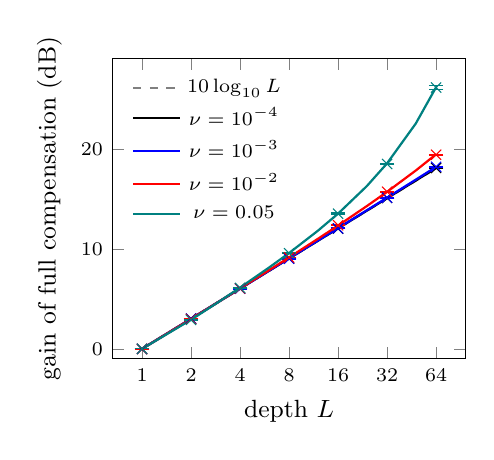
\begin{tikzpicture}
\begin{axis}[width=0.5\textwidth,height=5.4cm,xmode=log,log basis x=2,xlabel={depth $L$},ylabel={gain of full compensation (dB)},
legend style={font=\scriptsize,at={(0.03,0.97)},anchor=north west,draw=none,fill=none},xtick={1,2,4,8,16,32,64},xticklabels={1,2,4,8,16,32,64},tick label style={font=\scriptsize},label style={font=\small},ymin=-1]
\addplot[gray,dashed,thick] coordinates {(1,0) (2,3.0103) (3,4.77121) (4,6.0206) (6,7.78151) (8,9.0309) (12,10.7918) (16,12.0412) (24,13.8021) (32,15.0515) (48,16.8124) (64,18.0618)};
\addlegendentry{$10\log_{10}L$}
\addplot[black,thick] coordinates {(1,0) (2,3.01008) (3,4.77121) (4,6.02082) (6,7.78216) (8,9.03199) (12,10.7938) (16,12.044) (24,13.8067) (32,15.0578) (48,16.8222) (64,18.0751)};
\addlegendentry{$\nu=10^{-4}$}
\addplot[black,only marks,mark=x,mark size=2.6pt,forget plot,error bars/.cd,y dir=both,y explicit] coordinates {(1,-0.0246986) +- (0,0.0203) (2,3.01808) +- (0,0.0237) (4,6.03606) +- (0,0.0245) (8,9.04952) +- (0,0.0297) (16,12.0254) +- (0,0.0302) (32,15.0812) +- (0,0.026) (64,18.0805) +- (0,0.0389)};
\addplot[blue,thick] coordinates {(1,0) (2,3.00813) (3,4.77121) (4,6.02277) (6,7.78803) (8,9.04176) (12,10.8114) (16,12.0695) (24,13.8478) (32,15.1146) (48,16.9105) (64,18.1949)};
\addlegendentry{$\nu=10^{-3}$}
\addplot[blue,only marks,mark=x,mark size=2.6pt,forget plot,error bars/.cd,y dir=both,y explicit] coordinates {(1,0.00102925) +- (0,0.0187) (2,3.01757) +- (0,0.0245) (4,6.00769) +- (0,0.0255) (8,9.00679) +- (0,0.0265) (16,12.0452) +- (0,0.0308) (32,15.1101) +- (0,0.0325) (64,18.1993) +- (0,0.0363)};
\addplot[red,thick] coordinates {(1,0) (2,2.98875) (3,4.77093) (4,6.04204) (6,7.84653) (8,9.13963) (12,10.9884) (16,12.3262) (24,14.2657) (32,15.696) (48,17.8255) (64,19.4525)};
\addlegendentry{$\nu=10^{-2}$}
\addplot[red,only marks,mark=x,mark size=2.6pt,forget plot,error bars/.cd,y dir=both,y explicit] coordinates {(1,-0.00130742) +- (0,0.0206) (2,2.97385) +- (0,0.024) (4,6.04419) +- (0,0.0295) (8,9.13449) +- (0,0.0293) (16,12.3555) +- (0,0.0338) (32,15.7068) +- (0,0.0426) (64,19.4054) +- (0,0.0511)};
\addplot[teal,thick] coordinates {(1,0) (2,2.90565) (3,4.76433) (4,6.12216) (6,8.10355) (8,9.57686) (12,11.7959) (16,13.5169) (24,16.261) (32,18.5451) (48,22.5194) (64,26.1531)};
\addlegendentry{$\nu=0.05$}
\addplot[teal,only marks,mark=x,mark size=2.6pt,forget plot,error bars/.cd,y dir=both,y explicit] coordinates {(1,0.0106165) +- (0,0.0177) (2,2.89823) +- (0,0.0325) (4,6.09175) +- (0,0.0325) (8,9.55486) +- (0,0.042) (16,13.5196) +- (0,0.0558) (32,18.4774) +- (0,0.0823) (64,26.1215) +- (0,0.204)};
\end{axis}
\end{tikzpicture}
\caption{Gain as a function of depth in the class of Example~\ref{ex:iso}, $d=4$, with the actual algorithm and dithered rounding of the weights. Lines are the closed form; marks are simulations with two standard errors. Left: $\nu=10^{-2}$; circles, fixed teacher $W_l=I$ ($2\times10^4$ runs); crosses, random teachers ($100$ teachers, $200$ runs each, errors clustered by teacher). Right: ratio of the two errors, random teachers, with standard errors paired by teacher. At depth one the two schemes coincide.}\label{fig:gain}
\end{figure}
